\documentclass{report}
    \title{50003 - Models of Computation - Lecture 1}
    \author{Oliver Killane}
    \date{14/10/21}

%===========================COMMON FORMAT & COMMANDS===========================
% This file contains commands and format to be used by every module, and is 
% included in all files.
%===============================================================================

%====================================IMPORTS====================================
\usepackage[a4paper, total={6in, 8in}]{geometry}
\usepackage{graphicx, amssymb, amsfonts, amsmath, xcolor, listings, tcolorbox, multirow, hyperref}
%===============================================================================

%====================================IMAGES=====================================
\graphicspath{{image/}}

% \centerimage{options}{image}
\newcommand{\centerimage}[2]{\begin{center}
    \includegraphics[#1]{#2}
\end{center}}
%===============================================================================

%=================================CODE LISTINGS=================================
\definecolor{codebackdrop}{gray}{0.9}
\definecolor{commentgreen}{rgb}{0,0.6,0}
\lstset{
    inputpath=code, 
    commentstyle=\color{commentgreen},
    keywordstyle=\color{blue}, 
    backgroundcolor=\color{codebackdrop}, 
    basicstyle=\footnotesize,
    frame=single,
    numbers=left,
    stepnumber=1,
    showstringspaces=false,
    breaklines=true,
    postbreak=\mbox{\textcolor{red}{$\hookrightarrow$}\space}
}

% Create a code listing for a single line
% \codeline{language}{line}{file}
\newcommand{\codeline}[3]{\lstinputlisting[language=#1, firstline = #2, lastline = #2]{#3}}

% Create a code listing for a given language & file
% \codelist{language}{file}
\newcommand{\codelist}[2]{\lstinputlisting[language=#1]{#2}}
%===============================================================================

%================================TEXT STRUCTURES================================
% Marka a word as bold
% \keyword{important word}
\newcommand{\keyword}[1]{\textbf{#1}}

% Creates a section in italics
% \question{question in italics}
\newcommand{\question}[1]{\textit{#1} \\ }

% Creates a box with title for side notes.
% \sidenote{title}{contents}
\newcommand{\sidenote}[2]{\begin{tcolorbox}[title=#1]#2\end{tcolorbox}}

% Creates an item in an itemize or enumerate, with a paragraph after
% \begin{itemize}
%     \bullpara{title}{contents}
% \end{itemize}
\newcommand{\bullpara}[2]{\item \textbf{#1} \ #2}

% Creates a compact list (very small gaps between items)
% \compitem{
%     \item item 1
%     \item item 2
%     \item ...
% }
\newcommand{\compitem}[1]{\begin{itemize}\setlength\itemsep{-0.5em}#1\end{itemize}}

% Creates a link to the lecture for use at the start of the notes document
\newcommand{\lectlink}[1]{\sidenote{Lecture Recording}{
    Lecture recording is available \href{#1}{here}
}}
%===============================================================================


%================================CONFIGURATIONS================================
\newcommand{\config}[2]{\langle #1, #2 \rangle}
%==============================================================================

%==============================BIG STEP SEMANTICS==============================
\newcommand{\bigstep}[4]{\text{(#1)}\dfrac{#2}{#3 \Downarrow #4}}
\newcommand{\bigstepdef}[5]{\bigstep{#1}{#2}{#3}{#4} \ #5}
%==============================================================================

%=============================SMALL STEP SEMANTICS=============================
\newcommand{\smallstep}[4]{\text{(#1)}\dfrac{#2}{#3 \to #4}}
\newcommand{\smallstepdef}[5]{\smallstep{#1}{#2}{#3}{#4} \ #5}
%==============================================================================

\newcommand{\whilest}[3]{\text{(#1)}\dfrac{#2}{#3}}
\newcommand{\whilestdef}[4]{\whilest{#1}{#2}{#3} \ #4}
%==============================================================================

%===================================COMMANDS===================================
\newcommand{\while}[2]{\text{while } #1 \text{ do } #2}
\newcommand{\cond}[3]{\text{if } #1 \text{ then } #2 \text{ else } #3}
\newcommand{\doret}[2]{\text{do } #1 \text{ return } #2}

\newcommand{\instrlabel}[1]{\text{\textcolor{teal}{$L_{#1}$}}}
\newcommand{\reglabel}[1]{\text{\textcolor{orange}{$R_{#1}$}}}
\newcommand{\regtemp}[1]{\text{\textcolor{orange}{$#1$}}}
\newcommand{\instr}[2]{\instrlabel{#1} : & #2 \\}
\newcommand{\dec}[3]{\reglabel{#1}^- \to \instrlabel{#2}, \instrlabel{#3}}
\newcommand{\inc}[2]{\reglabel{#1}^+ \to \instrlabel{#2}}
\newcommand{\halt}{\text{\textcolor{red}{\textbf{HALT}}}}

\newcommand{\lambapp}[2]{#1 \ #2}
\newcommand{\lambappb}[2]{(#1) \ (#2)}
\newcommand{\lambfun}[2]{\lambda #1 \ . \ #2}

\makeatletter
\newcommand{\lambarg}[1]{%
	#1 \checknextarglambarg}
\newcommand{\checknextarglambarg}{\@ifnextchar\bgroup{\gobblenextarglambarg}{}}
\newcommand{\gobblenextarglambarg}[1]{ \ #1 \@ifnextchar\bgroup{\gobblenextarglambarg}{}}

\newcommand{\chnum}[1]{\underline{#1}}
% Variable argument regconfig \regconfig{label no}{reg val}{reg val}...
\makeatletter
\newcommand{\regconfig}[2]{%
	$#1$ & $#2$\checknextarg}
\newcommand{\checknextarg}{\@ifnextchar\bgroup{\gobblenextarg}{\\}}
\newcommand{\gobblenextarg}[1]{ & $#1$\@ifnextchar\bgroup{\gobblenextarg}{\\}}
%==============================================================================

\newcommand{\cenqu}[1]{\begin{center}\textit{#1}\end{center}}

\begin{document}
    \maketitle
    \lectlink{https://imperial.cloud.panopto.eu/Panopto/Pages/Viewer.aspx?id=ac0f6548-4293-4e26-905f-adbe00bc59ef}

    \section*{Course Admin}
        \subsection*{Part 1 - Azalea Raad (Week 2 - Week 6)}
            \begin{itemize}
                \bullpara{8 Virtual Lectures - Teams \& Recorded}{
                    Monday (11:00 - 12:00) \\
                    Friday (16:00 - 17:00)
                }
                \bullpara{4 Hybrid tutorials - Teams \& In Person}{
                    Friday (17:00 - 18:00)
                }
                \bullpara{1 Bonus Hour - Teams \& Recorded}{
                    Monday 8/11/2012
                }
            \end{itemize}
            We will cover:
            \begin{itemize}
                \item Operational Semantics of a small while language
                \item Denotational semantics of a small while language (notes only)
                \item Register machines, universal register machine, Halting problem.
                \item Turing machines and Turing computable functions, primitive and partial recursive functions
                \item Lambda calculus and equivalence results.
            \end{itemize}
        \subsection*{Part 2 - Herbert Wiklicky (Week 6 - Week 10)}
            \begin{itemize}
                \bullpara{Hybrid Lectures - Teams \& In Person \& Recorded}{
                    Friday (16:00 - 18:00)
                }
                \bullpara{Virtual Tutorials - Teams}{
                    Monday (11:00 - 12:00)
                }
            \end{itemize}
    \section*{Algorithms}
        \subsubsection*{Examples of Algorithms}
            \begin{itemize}
                \bullpara{Euclid's Algorithm $\approx$300 B.C. }{
                    Algorithm to find the greatest common divisior.
                    \lstinputlisting[language=Haskell]{euclid.hs}
                }
                \bullpara{Sieve of Eratosthenes $\approx$200 B.C.} {
                    Used to find the prime numbers within a limit. Done by starting from the 2, adding the number to the primes, then marking all multiples, then repeating progressing to the next non-marked number (a prime), marking all multiples and repeating.
                    \lstinputlisting[language=Haskell]{sieve of eratosthenes.hs}
                }
                \bullpara{Well-Known Rules for $+ - \div \times$  $\approx$900 A.D.}{
                    Al-Khwarizmi, a persian mathematician who was appointed astronomer and head of the library in the Bagdad House of Wisdom.
                }
                \bullpara{Simple Machines using punchcards. Mainly 19th Century}{
                    Weaving looms, pianola, census tabulating machine.
                }
                \bullpara{Analytical Engine}{
                    A proposed multi-purpose calculating machine designed by Charles Babbage. Using a simple ALU, with conditional branching and integrated memory. As a result the first Turing complete computer.
                    \\
                    \\ First ever program was written by Ada Lovelace to calculate the Bernoulli numbers.
                }
            \end{itemize}

        \subsubsection{Decision Problems}
            Given:
            \begin{itemize}
                \item A set $S$ of finite data structures of some kind (e.g formulae in first order logic).
                \item A property $P$ of elements of $S$ (e.g the porperty of a formula that it has a proof).
            \end{itemize}
            \sidenote{Formulas} {Well formed logical statements that are a sequence of symbols form a given formal language. e.g $(p \lor q) \land i$ is a formula, but $) \lor \land j i$ is not.}
            The associated decision procedure is:
            \\
            \\ Find an algorithm such that for any $s \in S$, if $s$ has property $P$ the algorithm terminates with $1$, otherwise with $0$.
        
        \subsubsection*{Hilbert's Entscheidungsproblem}
            \cenqu{Is there an algorithm which can take any statement in first-order logic, and determine in a finite number of steps if the statement is provable?}

            \sidenote{First Order Logic}{Also called predicate logic, is an extension of propositional logic that includes quanifiers ($\forall, \exists$), equality, function symbols (e.g $\times, \div, +, -$) and structured formulas (predicate functions).}
            
            This problem was originally presented in a more ambiguous form, using a logic system more powerful than first-order.
            \\
            \\ '\textit{Entscheidungsproblem}' means 'decision problem'
            \\
            \\ Many tired to solve the porblem, without success. One strategy was to try and disprove that such an algorithm can exist. 
            In order to answer this question properly a formal definiotion of algorithm was required.
        
        \subsubsection*{Algorithms Informally}
            Common features of Algorithms:
            \begin{itemize}
                \bullpara{Finite}{
                    Description of the procedure in terms of elementary operations.
                }
                \bullpara{Deterministic}{
                    If there is a next step, it is uniquely determined - that is on the same data, the same steps will be made.
                }
                \bullpara{Maybe Terminate}{
                    procedure may not terminate on some input data, however we can recognise when it terminates and what the result is.
                }
            \end{itemize}

            In 1935/35, Alan Turing (Cambridge) and Church (Princeton) independently gave negative soltuions to Hilberts Entscheidungsproblem (showed such an algorithm could not exist).
            \begin{enumerate}
                \item They gave concrete/precise definitions of what algorithms are (Turing Machines \& Lambda Calculus).
                \item They regarded algorithms as data, on which other algorithms could act.
                \item They reduced the problem to the \keyword{Halting problem}.
            \end{enumerate}
            This work led to the Church-Turing Thesis, that shows everything computable is computed by a Turing Machine. Church's Thesis extended this to show that General Recurisve Functions were the same type as those expressed by lambda calculus, and Turning showed that lambda calculus and the turning machine were equivalent.
        \subsubsection*{Algorithms Formalised}
            Any formal definition of an algorithm should be:
            \begin{itemize}
                \bullpara{Precise}{
                    No ambiguities, no implicit assumptions, Should be phrased mathematically.
                }
                \bullpara{Simple}{
                    No unnecessary details, only the few axioms required. Makes it easier to reason about.
                }
                \bullpara{General}{
                    So all algorithms and types of algorithms are covered.
                }
            \end{itemize}
        \subsubsection*{The Halting Problem}
            The \keyword{Halting problem} is a decision problem with:
            \begin{itemize}
                \item The set of all pairs $(A,D)$ such that $A$ is an algorithm, and $D$ is some input datum on which the algorithm operates.
                \item The property $A(D)\downarrow$ holds for $(A,D) \in S$ if algorithm $A$ when applied to $D$ eventually produces a result (halts).
            \end{itemize}
            Turning and Church showed that there is no algorithm such that:
            \[\forall (A,D) \in S \begin{bmatrix}
                H (A,D) & = & 1 & A(D)\downarrow \\
                & & 0 & otherwise
            \end{bmatrix}\]
            The final step for Turing/Church's proof was to construct an algorithm encoding instances $(A,D)$ of the halting problem as statements such that:
            \[\Phi_{A,D} \ is \ provable \leftrightarrow A(D)\downarrow\]
        
        \subsubsection*{Algorithms as Functions}
            It is possible to give a mathematical description of a computable function as a special function between special sets.
            \\
            \\ In the 1960s Strachey \& Scott (Oxford) introduced \keyword{denotational semantics}, which describes tje meaning (denotation)
            of an algorithm as a function that maps input to output.
            \sidenote{Domains}{
                Domains are special kinds of partially ordered sets. Partial orders meaning there is an order of elements in the set, but not every element is comparable.
                \\
                \\ Partial orders are reflexive, transitive and anti-symmetric. You can easily represent them on a Hasse Diagram.
                \begin{center}
                    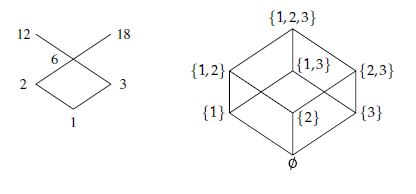
\includegraphics{hasse diagram.png}
                \end{center}
            }
            Scott solved the most difficult part, considering recursively defined algorithms as continuous functions between domains.


        \subsubsection*{Haskell Programs}
            Example using a basic implementation of power.
            \codelist{Haskell}{power.hs}

            \newcommand{\step}[1]{$\leadsto$ \ #1\\}
            
            \begin{minipage}{.5\textwidth}
                \textbf{O(n)} \\
                power 7 5 \\
                \step{7 * (power 7 4)}
                \step{7 * ( 7 * (power 7 3))}
                \step{7 * ( 7 * (7 * (power 7 2)))}
                \step{7 * ( 7 * (7 * (7 * (power 7 1))))}
                \step{7 * ( 7 * (7 * (7 * (7 * (power 7 0)))))}
                \step{7 * ( 7 * (7 * (7 * (7 * 1))))}
                \step{16807}
            \end{minipage} \begin{minipage}{.5\textwidth}
                \textbf{O(log(n)) steps} \\
                power' 7 5 \\
                \step{7 * (power' 7 2)\^2}
                \step{7 * ((power' 7 1)\^2)\^2}
                \step{7 * ((7 * (power' 7 0)\^2)\^2)\^2}
                \step{7 * ((7 * (1)\^2)\^2)\^2}
                \step{16807}
            \end{minipage}

            These two functions are equivalent in result however operate differently (one much faster than the other).

        \subsubsection*{Program Semantics}
            \textbf{Denotational Semantics:}
            \begin{itemize}
                \item A program's meaning is described compositionally using denotations (mathematical objects)
                \item A denotation of a program phrase is built from its subphrases.
            \end{itemize}
            \textbf{Operational Semantics:}
            \begin{itemize}
                \item Program's meaning is given in terms of the steps taken to make it run.
            \end{itemize}
            There is also \keyword{axiomatic semantics} and \keyword{declarative semantics} but we will not cover them.
\end{document}
